\documentclass{article}

\usepackage{graphicx}
\usepackage{hyperref}
\usepackage{amsmath}
\usepackage{amssymb}
\usepackage{blkarray}
\usepackage{cancel}
\usepackage{fancyhdr}
\usepackage{enumitem}
\usepackage{lscape}
\usepackage{listings}
\usepackage{color}
\usepackage{pdfpages}
\usepackage{yfonts}

\definecolor{dkgreen}{rgb}{0,0.6,0}
\definecolor{gray}{rgb}{0.5,0.5,0.5}
\definecolor{mauve}{rgb}{0.58,0,0.82}

\usepackage{xcolor}

\lstdefinestyle{base}{
  inputencoding=latin10,
  emptylines=1,
  breaklines=true,
  basicstyle=\small\ttfamily,
  moredelim=**[is][\color{red}]{@}{@},
}

\newcommand{\norm}[1]{\left\lVert#1\right\rVert}

%% Define a HUGE 
\makeatletter
\newcommand\HUGE{\@setfontsize\Huge{50}{60}}
\makeatother

\begin{document}             % End of preamble and beginning of text.

 
%titlepage
\thispagestyle{empty}
\begin{center}
\begin{minipage}{.9\linewidth}
\flushright
	      		 

\includegraphics[width=0.5\linewidth]{univie.jpg}\par
\vspace{1.5cm}
\centering 	
    % Title
	{\scshape{\HUGE A4 Report \par}}
	\vspace{1cm}
	%Thesis title
    {\scshape{\Large Course: VIS WS '18 \par}}
	\vspace{1cm}

 {\Large Name : Robert Ernstbrunner \\ Matnr.: 01403753 \hspace{2.2cm} \ \par}
 	\vspace{.7cm}

 

\end{minipage}
\end{center}
\clearpage
\section{Introduction}

The ornithology student \textit{Mitch Vogel} needs our help in visualizing his data in order to advance in his investigations. There is an observed decline in the nesting \textit{Rose-crested Blue Pipit} in the \textit{Boonsong Lekagul Nature Preserve} and Mitch thinks the traffic going through the preserve might have to do with it.
He reckons that traffic noise might overshadow mating calls or that invading campers might scare away the birds from their habitat areas. \\
The data was collected by park Rangers who work as caretakers of the nature preserve. They gave Mitch additional explanations about the data together with a map. 

\section{Data, Users, Tasks}
The park Rangers monitor the traffic through the preserve. They assign tickets to vehicles at the entry gates.
\begin{itemize}

\item In summary there are seven different types of vehicles:

	\begin{enumerate}
	\item \textit{Cars} and \textit{motorcycles} count as one type.
	\item There are three different types of \textit{trucks} (differentiated by their number of axles).
	\item There are two types of \textit{buses}.
	\item The seventh type consists of \textit{park service trucks} that are used by the Rangers who have access to all areas.
	\end{enumerate}

\item There are five different types of sensors:

	\begin{enumerate}
	\item Vehicles that enter or leave the preserve are tracked at \textit{entrance gates}.
	\item \textit{General gates} act as control points to monitor the traffic flow.
	\item Special gates that are simply referred to as \textit{gates} are there to prevent general traffic from passing. These gates can only be opened by Rangers.
	\item \textit{Ranger-stops} represent the working areas for Rangers. Some are cut off from general traffic and some aren't. That's why some of their sensors also collect general traffic information while the others don't.
	\item Finally \textit{camping} sensors monitor visitors, that enter or exit a camping ground.
	\end{enumerate}

\item Additional information about the dataset:

	\begin{enumerate}		
	\item Traffic either passes through the preserve, stay as day campers or stay as extended campers.
	\item Rangers reside at the southeast Ranger-stop when they are not working.
	\item The speed limit is 25 mph.
	\item Summertime is not included in the sensor measurements.
	\item Traffic going southward from entrance gates \textit{three} and \textit{four} are not represented on the map and are not tracked.
	\end{enumerate}

\item Data snippet:\\
\noindent\rule{9.3cm}{1pt}\\
\texttt{Timestamp,car-id,car-type,gate-name}\\
\texttt{2015-05-01 00:15:13,20151501121513-39,2,entrance4}\\
\texttt{2015-05-01 00:32:47,20151501121513-39,2,entrance2}\\
\texttt{2015-05-01 01:12:42,20151201011242-330,5,entrance0}\\
\noindent\rule{9.3cm}{1pt}\\

The data set consists of the following parameters:

	\begin{enumerate}
	\item \textit{Timestamp} \textcolor{red}{(quantitative)} contains the date and time the sensor was triggered.
	\item Entering vehicles are assigned with a \textit{car-ID} \textcolor{olive}{(nominal)} at the \textit{entry gates}.
	\item The \textit{Car-type} \textcolor{olive}{(nominal)} specifies a vehicle according to their type and number of axles. A park vehicle gets additionally marked with a \textit{'P'}.
	\item The \textit{Gate-name} \textcolor{olive}{(nominal)} is the name of the sensors themselves. The same names can also be found on the map.
	\end{enumerate}

\item The map:
	
	\begin{center}
	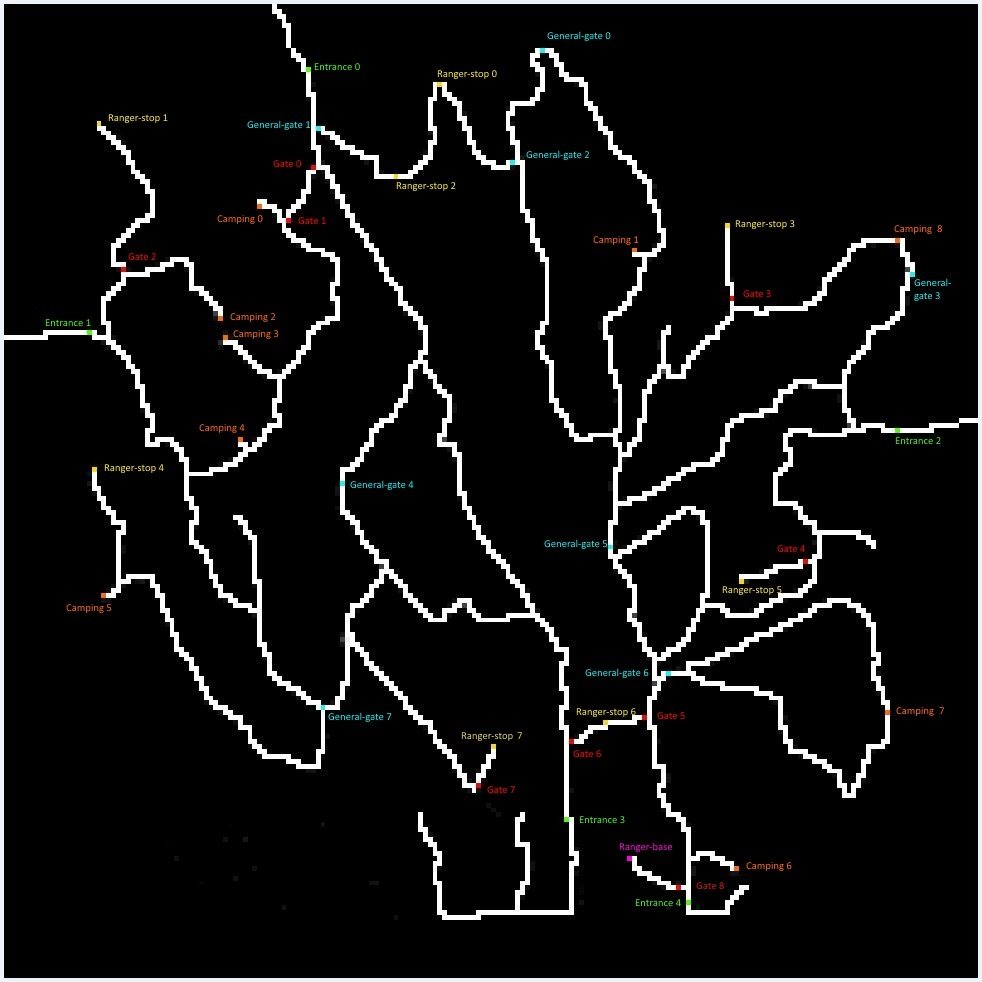
\includegraphics[scale=0.3]{Lekagul_Roadways_labeled_v2.jpg}	
	\end{center}
	
	The map consists of a simple black background with white roads and type-colored gate labels. It may be used by the flow map visualization (design 2).
\item The preserve:

\end{itemize}

\section{Designs}
\subsection{examine correlation of durations}
\begin{center}
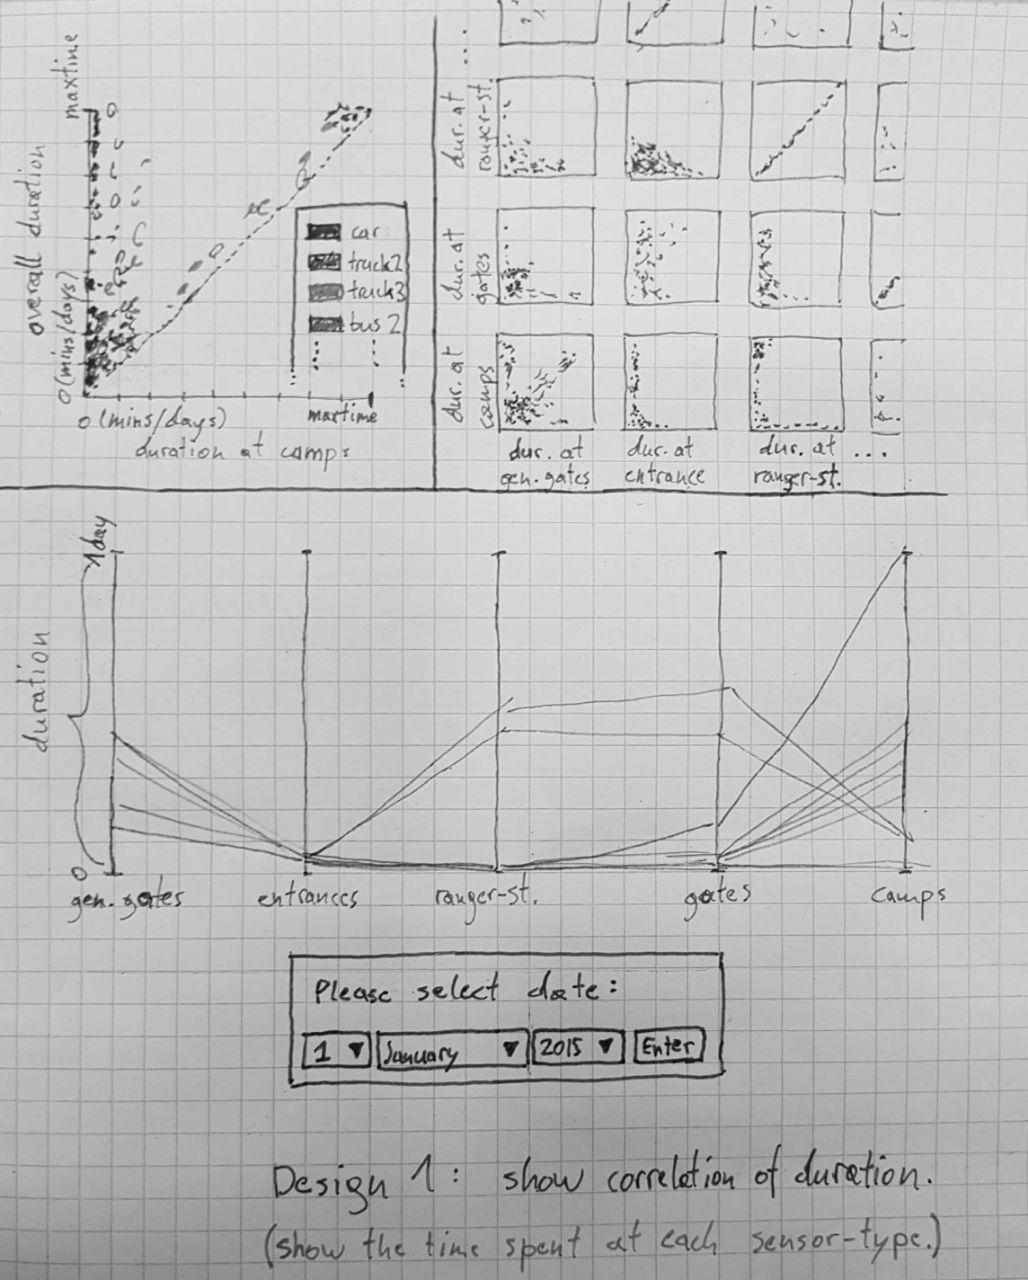
\includegraphics[scale=.5]{Design1.jpg}
\end{center}

\subsection{visualize traffic flow}

\begin{center}
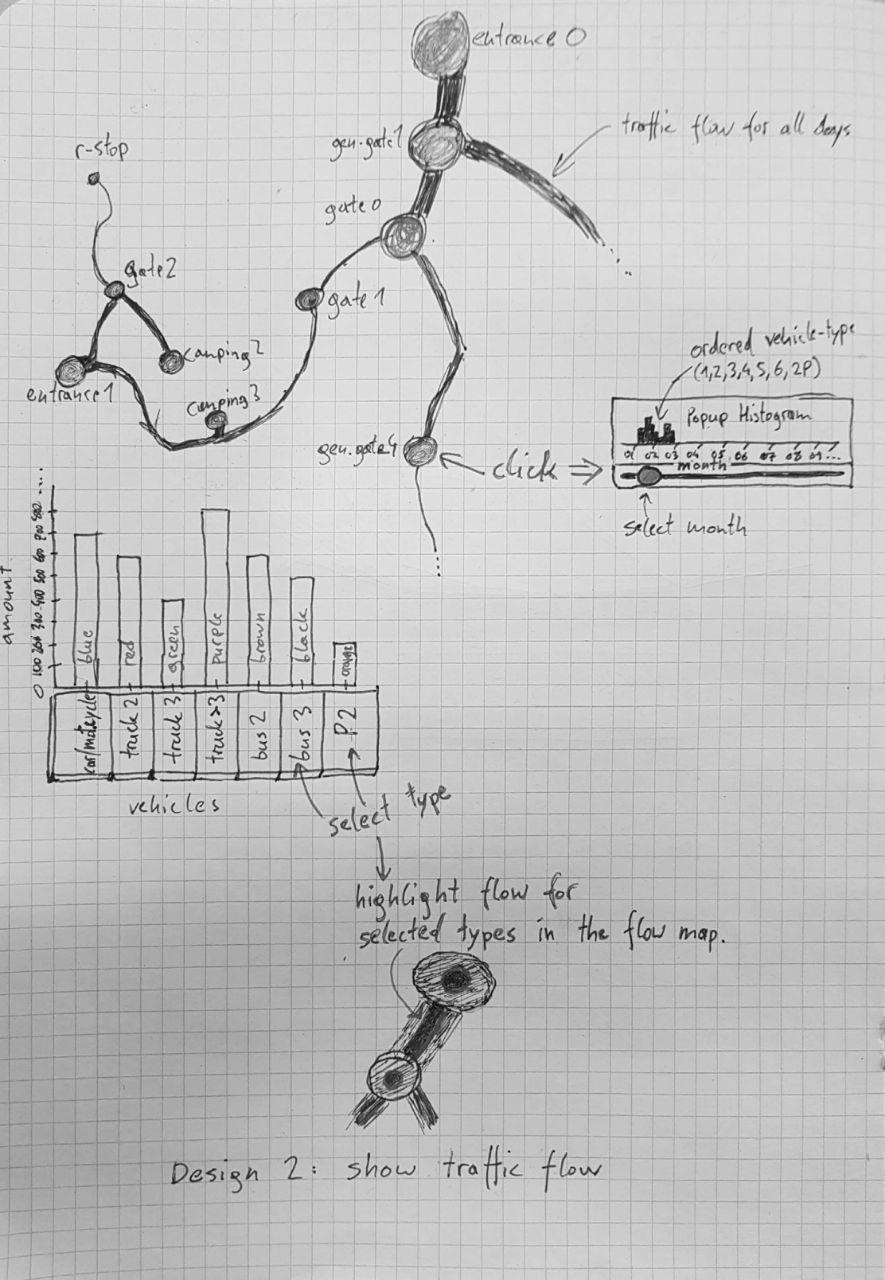
\includegraphics[scale=0.65]{Design2.jpg}	
\end{center}

\section{Summary}
\subsection{task abstraction}
I noticed that only arrivals at gates / camps are tracked, but no departures. Therefore, we could come up with the assumption, that campers could also camp somewhere along the way before the next gate. However, in the Lekagul Preserve description file, it clearly states, that camping and cycling are only allowed in designated areas. So if the Rangers do their job properly, (which we could check by visualization) it is reasonable to strongly assume the opposite.\\

Also, there is no information about the birds themselves. This fact limits the visualization space by narrowing the visualization tasks to the traffic only.

\subsection{Visual encoding}
Flow map works good for visualizing the movements of objects from one location to another. spacial density of traffic. Flow maps reduce visual clutter by merging edges. 



\begin{thebibliography}{9}

\bibitem{nothing}
\url{https://}

\end{thebibliography}

\end{document}
% End of document.